\documentclass[xcolor=x11names,compress,professionalfonts]{beamer}

%% General packages %%%%%%%%%%%%%%%%%%%%%%%%%%%%%%%%%%
\usepackage[utf8]{inputenc}
\usepackage{graphicx}
\usepackage{tikz}
\tikzset{% change default arrow tips
    >=latex
}
\usepackage{ifthen}

\usepackage{amsmath}
\usepackage{nicefrac}

\usepackage{color}

%%%%%%%%%%%%%%%%%%%%%%%%%%%%%%%%%%%%%%%%%%%%%%%%%%%%%%


%% Beamer Layout %%%%%%%%%%%%%%%%%%%%%%%%%%%%%%%%%%
\useoutertheme[subsection=false,shadow]{miniframes}
\useinnertheme{rectangles}

\setbeamertemplate{navigation symbols}{}%remove navigation symbols

\usepackage{libertine}
\usepackage[T1]{fontenc}

\setbeamerfont{title like}{shape=\scshape}
\setbeamerfont{frametitle}{shape=\scshape}

\setbeamercolor*{lower separation line head}{bg=DeepSkyBlue4} 
\setbeamercolor*{normal text}{fg=black,bg=white} 
\setbeamercolor*{alerted text}{fg=red} 
\setbeamercolor*{example text}{fg=black} 
\setbeamercolor*{structure}{fg=black} 
 
\setbeamercolor*{palette tertiary}{fg=black,bg=black!10} 
\setbeamercolor*{palette quaternary}{fg=black,bg=black!10} 

\renewcommand{\(}{\begin{columns}}
\renewcommand{\)}{\end{columns}}
\newcommand{\<}[1]{\begin{column}{#1}}
\renewcommand{\>}{\end{column}}

\newcommand{\om}{\ensuremath{\omega}}
\newcommand{\lb}{\ensuremath{\overline{\lambda}}}
\newcommand{\zb}{\ensuremath{\overline{z}}}
\newcommand{\ham}{\ensuremath{H}}

\definecolor{BostonBlue}{HTML}{00688B}
\definecolor{Complementary}{HTML}{8B2300}
%%%%%%%%%%%%%%%%%%%%%%%%%%%%%%%%%%%%%%%%%%%%%%%%%%

\usepackage{braket}
% compile child documents using this preamble
\usepackage{subfiles}

%%%My Math

\newcommand{\pd}[2]{\frac{\displaystyle \partial #1}{\displaystyle\partial #2}} % for partial derivatives
\newcommand{\dx}{\mathrm{d}x}
\renewcommand{\d}[1]{\mathrm{d}#1}
\newcommand{\nth}{$n^\text{th}$ }

\newcommand{\mean}[1]{\langle #1 \rangle}
\DeclareMathOperator{\Pf}{Pf}
\DeclareMathOperator{\Tr}{Tr}

\begin{document}


\begin{frame}
\title{Fractal dimensions of the Fibonacci chain}
%\subtitle{SUBTITLE}
\author{ Nicolas Macé, Anuradha Jagannathan, Frédéric Piéchon }
\date{
	June 24, 2015
}
\titlepage
\end{frame}

\section{Electronic properties of the Fibonacci chain.}
%Each section needs a subsection for the small points on top to show up
\subsection{Dummy}

\begin{frame}{The model: the Fibonacci chain}
	\centering
	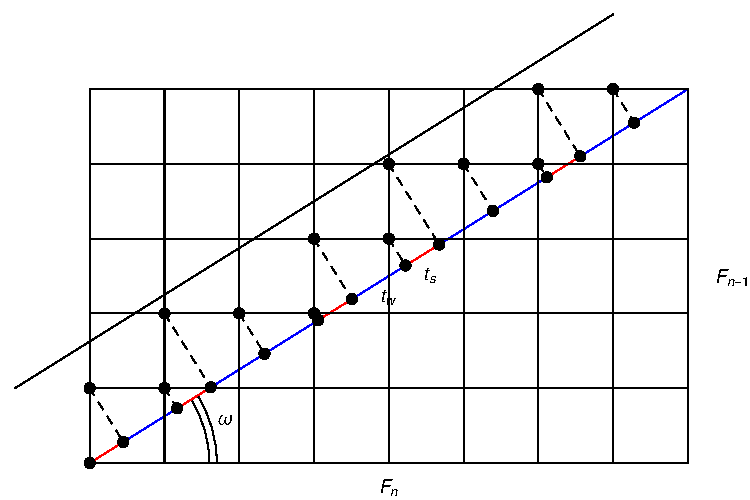
\includegraphics[scale=.7]{cut_and_project.pdf}
	\[ \ham_n = - \sum t_i^{(n)} \ket{i} \bra{i} \]
\end{frame}

\begin{frame}{Atoms \& molecules; deflation}
	\centering
	\begin{itemize}
	\item Atomic deflation \subfile{atomic_deflation.tex}
	\item Molecular deflation \subfile{molecular_deflation.tex}
	\end{itemize}
	RG transformation $(\ham_n, t_s, t_w) \rightarrow (\ham_{n-3}, \ham_{n-2}, \ham_{n-2}, t_s', t_w')$
\end{frame}

\begin{frame}{Renormalization group}
\end{frame}

\begin{frame}{Recursive construction of the spectrum}
\end{frame}

\begin{frame}{Fractal dimensions}
\end{frame}

\begin{frame}{Fractal dimensions of the wavefunctions}
\end{frame}

\begin{frame}{Multifractality of the Fibonacci chain}
\end{frame}

\begin{frame}{Local multifractality}
\end{frame}

\begin{frame}{Conumbering}
\end{frame}

\begin{frame}{Conumbering in the strong quasiperiodic limit}
\end{frame}

\begin{frame}{Gap labelling \& conumberings}
\end{frame}

\end{document}
